% !TEX program = pdflatex
% arara: pdflatex: { shell: false }
% arara: pdflatex: { shell: false }
% arara: latexmk: { options: ["-c"] }
% -------------------------------
\input{inc/_m.latex}
\input{inc/_ev.latex}
% -------------------------------
\nc{\Classe}{2nde}
\nc{\Titre}{Probabilité / Vecteur et colinéarité}
\nc{\EvalTotal}{20}
% -------------------------------

\begin{document}
% -------------------------------
\begin{exo}{Alignement}{4}
	\begin{wrapfigure}{r}{6cm}
		\begin{center}
			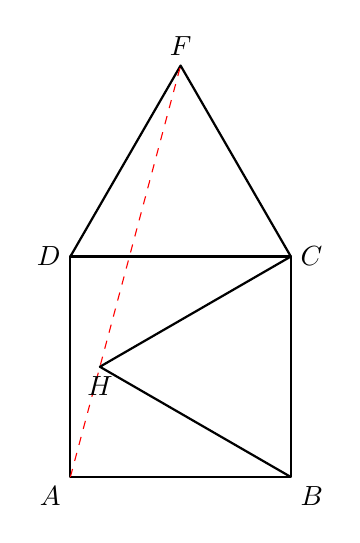
\begin{tikzpicture}[scale=0.7, line join=round]
				% Définition des points du carré (côté 4cm)
				\coordinate (A) at (0,0);
				\coordinate (B) at (4,0);
				\coordinate (C) at (4,4);
				\coordinate (D) at (0,4);

				% Tracé du carré
				\draw[thick] (A) -- (B) -- (C) -- (D) -- cycle;

				% Triangle équilatéral DFC (vers le haut)
				% La hauteur est 4 * sin(60°) = 2*sqrt(3)
				\coordinate (F) at (2,{4 + 2*sqrt(3)});
				\draw[thick] (D) -- (F) -- (C);

				% Triangle équilatéral BCH (vers l'intérieur)
				% La pointe H est à 4 - 2*sqrt(3) du bord droit
				\coordinate (H) at ({4 - 2*sqrt(3)}, 2);
				\draw[thick] (B) -- (H) -- (C);

				% Tracé de la ligne pour démontrer l'alignement (A, H, F)
				\draw[dashed, red] (A) -- (F);

				% Étiquettes des points
				\node[below left] at (A) {$A$};
				\node[below right] at (B) {$B$};
				\node[right] at (C) {$C$};
				\node[left] at (D) {$D$};
				\node[above] at (F) {$F$};
				\node[below] at (H) {$H$};
			\end{tikzpicture}
		\end{center}
	\end{wrapfigure}
	$ABCD$ est un carré de côté $4$ cm.\\ $DFC$ et $BCH$ sont des triangles équilatéraux.
	\begin{enumerate}[leftmargin=*]
		\q{1} Calculer la hauteur de chaque triangle.
		\q{1} Démontrer que les points $A, H$ et $F$ sont alignés.
	\end{enumerate}
	\vspace*{5cm}
\end{exo}
% -------------------------------
\newpage
% -------------------------------
\begin{exo}{}{5}
	PLOP
	\be[leftmargin=*]
	\q{2} mais pourquoi ?
	\q{2} mais pourquoi ?
	\q{2} mais pourquoi ?
	\ee
\end{exo}
% -------------------------------
\end{document}
